\documentclass[12pt,a4paper]{article}
\usepackage{fontenc}
\usepackage[english]{babel}
\usepackage[left=2cm,right=2cm,top=2.5cm,bottom=2.7cm]{geometry}
\usepackage{amsmath}
\usepackage[labelfont=bf]{caption}
\usepackage{tabularx}

\usepackage{indentfirst}
\usepackage{setspace}
\usepackage[linesnumbered,ruled]{algorithm2e}



% encrypt content from copying
%\usepackage{fancyvrb}
%\usepackage[resetfonts]{cmap}
%\begin{VerbatimOut}{ot1.cmap}
%	%!PS-Adobe-3.0 Resource-CMap
%	%%DocumentNeededResources: ProcSet (CIDInit)
%	%%IncludeResource: ProcSet (CIDInit)
%	%%BeginResource: CMap (TeX-OT1-0)
%	%%Title: (TeX-OT1-0 TeX OT1 0)
%	%%Version: 1.000
%	%%EndComments
%	/CIDInit /ProcSet findresource begin
%	12 dict begin
%	begincmap
%	/CIDSystemInfo
%	<< /Registry (TeX)
%	/Ordering (OT1)
%	/Supplement 0
%	>> def
%	/CMapName /TeX-OT1-0 def
%	/CMapType 2 def
%	1 begincodespacerange
%	<00> <7F>
%	endcodespacerange
%	8 beginbfrange
%	<00> <01> <0000>	<09> <0A> <0000>	<23> <26> <0000>
%	<28> <3B> <0000>	<3F> <5B> <0000>	<5D> <5E> <0000>
%	<61> <7A> <0000>	<7B> <7C> <0000>
%	endbfrange
%	40 beginbfchar
%	<02> <0000>	<03> <0000> <04> <0000> <05> <0000>
%	<06> <0000>	<07> <0000>	<08> <0000>	<0B> <0000>
%	<0C> <0000>	<0D> <0000>	<0E> <0000>	<0F> <0000>
%	<10> <0000>	<11> <0000>	<12> <0000>	<13> <0000>
%	<14> <0000>	<15> <0000>	<16> <0000>	<17> <0000>
%	<18> <0000>	<19> <0000>	<1A> <0000>	<1B> <0000>
%	<1C> <0000>	<1D> <0000>	<1E> <0000>	<1F> <0000>
%	<21> <0000>	<22> <0000>	<27> <0000>	<3C> <0000>
%	<3D> <0000>	<3E> <0000>	<5C> <0000>	<5F> <0000>
%	<60> <0000>	<7D> <0000>	<7E> <0000>	<7F> <0000>
%	endbfchar
%	endcmap
%	CMapName currentdict /CMap defineresource pop
%	end
%	end
%	%%EndResource
%	%%EOF
%\end{VerbatimOut}

% for a fancy header and footer
\newcommand\authorName{Nguyen The Anh - 52100744}
\newcommand{\email}{52100744@student.tdtu.edu.vn}
\newcommand\titleName{A study of Optimization Methods, \\ Continual Learning, and Test Production 
	in building Machine Learning Solutions}
\newcommand\mainHeader{Machine Learning}
\newcommand\subHeader{Final report}

\setlength{\headheight}{20pt}
\usepackage{fancyhdr}
\pagestyle{fancy}
\fancyhead[L]{\textbf{\large{\mainHeader}}}
\fancyhead[R]{\subHeader}
\fancyfoot[L]{\email}
\renewcommand{\footrulewidth}{0.3pt}

% Redefine the first page style
\fancypagestyle{plain}{%
	\fancyhf{}%
	\fancyhead[L]{\textbf{\large{\mainHeader}}}
	\fancyhead[R]{\subHeader}
	\fancyfoot[C]{\thepage}
	\fancyfoot[L]{\authorName}%
	\renewcommand{\headrulewidth}{0.4pt}% Line at the header invisible
	\renewcommand{\footrulewidth}{0.3pt}% Footer line not visible with 0pt
}

% adjust the \tab
\newcommand\tab[1][1cm]{\hspace*{#1}}


\author{\textit{\authorName}}
\title{\textbf{\titleName}}

% inserting image
\usepackage{graphicx}
\graphicspath{{./images/}}

% clickable table of contents
\usepackage{hyperref}
\hypersetup{
	linktoc=all,     %set to all if you want both sections and subsections linked
}

% for coding
\usepackage{listings}
\usepackage{color}

\definecolor{dkgreen}{rgb}{0,0.6,0}
\definecolor{gray}{rgb}{0.5,0.5,0.5}
\definecolor{mauve}{RGB}{128, 0, 0}
\definecolor{bg}{RGB}{230, 209, 149}


\lstset{frame=tb,
	language=Python,
	aboveskip=3mm,
	belowskip=3mm,
	showstringspaces=false,
	columns=flexible,
	basicstyle={\small\ttfamily},
	numbers=left,
	numberstyle=\tiny\color{gray},
	keywordstyle=\color{blue},
	commentstyle=\color{dkgreen},
	stringstyle=\color{mauve},
	breaklines=true,
	breakatwhitespace=true,
	tabsize=4
}

% note section configuration
\usepackage[most]{tcolorbox}
\makeatletter
\NewDocumentCommand{\note}{+O{}+m}{%
	\vspace{0.3cm}
	\begin{tcolorbox}[width=6.2in,
		enhanced,
		sharp corners,
		toprule=0pt,
		bottomrule=0pt,
		leftrule=5pt,
		rightrule=0pt,
		colback=red!20,
		colframe=red!80,
		#1
		]
		#2
	\end{tcolorbox}
}
\makeatother

\begin{document}
	\maketitle
	\numberwithin{figure}{section}
	

\section{Optimization methods}

The goal of machine learning is to find the optimal function \(f(x)\) to minimize the loss function on the training dataset. This means that our model needs to learn how to map the input \(x\) to the output \(f(x)\) in order to minimize the value of the loss function. This process often involves updating the model's weights through the use of \textit{optimization methods}. In other words, the objective of this process is to find weight values that can minimize the error between the model's predicted values and the actual values (loss) as much as possible.

Optimization methods in machine learning can be categorized into three types: first-order optimization, high-order optimization, and derivative-free optimization \cite{optimization}.


\subsection{First-order optimization methods}
The optimization methods in this category primarily rely on first derivative (gradient) of the loss function with respect to the parameters. Particularly, these methods include gradient descent, stochastic gradient descent, and adaptive learning rate.

\subsubsection{Gradient Descent}

The fundamental idea of the gradient descent method is to iteratively update variables in the opposite direction of the derivative of the objective function. The updates are performed to gradually converge to the optimal value of the objective function.

Specifically, in each iteration, the variables are updated according to the following formula:

\begin{equation}
	\theta_{i+1} = \theta_i - \eta \cdot \nabla J(\theta_i)
\end{equation}
, where:
\begin{itemize}
	\item \(\theta_{i+1}\) represents the updated parameter at iteration \(i+1\).
	\item \(\theta_i\) is the parameter at iteration \(i\).
	\item \(\eta\) is the learning rate.
	\item \(\nabla J(\theta_i)\) is the gradient of the objective function \(J\) with respect to the parameters \(\theta_i\).
\end{itemize}

The learning rate $(\eta)$ is a critical hyperparameter in the training process of machine learning models. It plays a pivotal role in controlling the magnitude of parameter updates during each iteration of optimization algorithms like gradient descent. Therefore, choosing a learning rate is an important step so we must \textit{choose it carefully}.


\begin{figure}[htb]
	\centering
	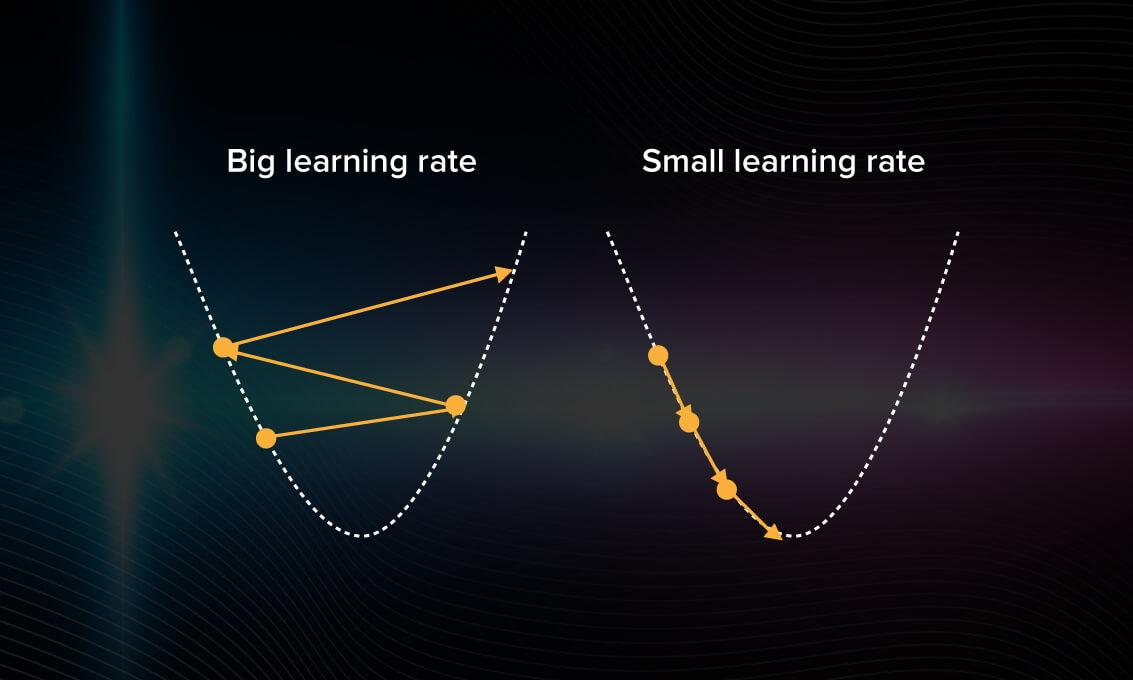
\includegraphics[width=0.7\linewidth]{assets/learning_rate}
	\caption{An example of choosing a large and small learning rate value.}
	\text{source: \url{ https://serokell.io/files/hq/hqopw87o.5\_(18)\_(1).jpg}}
	\label{fig:learningrate}
\end{figure}


When the learning rate is large, convergence may be faster initially but it increases the risk of overshooting the minimum, leading to divergence or oscillations. And when the learning rate is small, convergence is more stable, and the model is less likely to diverge but it may slow down the convergence process, requiring more iterations to reach the minimum.

Let's take linear regression model (demonstrated in the figure \ref{fig:linearregression}) as an example of the use of gradient descent. The linear regression model predicts the output $y$ based on input feature $x$ using the equation:
\begin{equation}
	h_\theta(x) = \theta_0 + \theta_1 x
\end{equation}
Here, $h_\theta(x)$ is the predicted output, $\theta_0$ is the y-intercept, $\theta_1$ is the slope, and $x$ is the input feature.

\begin{figure}
	\centering
	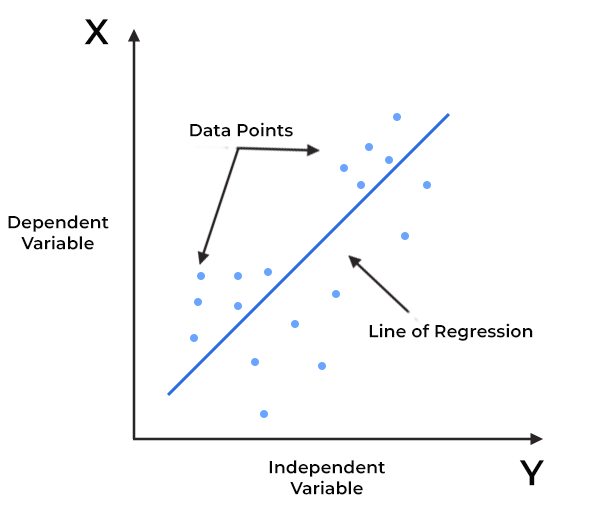
\includegraphics[width=0.5\linewidth]{assets/linear_regression}
	\caption{Linear Regression model is basically represented on graph}
	\text{source: \url{https://images.spiceworks.com/wp-content/uploads/2022/04/07040339/25-4.png}}
	\label{fig:linearregression}
\end{figure}


The model uses mean squares error (MSE) as the loss function. The function is formulated with the $i-th$ data point as:
\begin{equation}
	L_i(\theta) = \frac{1}{2} \left(h_\theta(x^{(i)}) - y^{(i)}\right)^2
\end{equation}

The total loss over the entire dataset is the average of these individual losses, where $n$ is the number of data points:
\begin{equation}
	 L(\theta) = \frac{1}{2n} \sum_{i=1}^{n} \left(h_\theta(x^{(i)}) - y^{(i)}\right)^2
\end{equation}

The update rule for gradient descent adjusts the parameters $\theta_0$ and $\theta_1$ to minimize the loss:
\begin{equation}
	\theta_j := \theta_j - \alpha \frac{1}{n} \sum_{i=1}^{n} \left(h_\theta(x^{(i)}) - y^{(i)}\right) x_j^{(i)}
\end{equation}
Here, $\alpha$ is the learning rate, $n$ is the number of data points, $j$ represents each parameter in the model, and $x_j^{(i)}$ is the $j$-th feature of the $i$-th data point.



When using the entire training data to compute the gradient of the cost function with respect to the model parameters in each iteration, and subsequently updating the parameters once per iteration based on the average gradient, is called \textit{batch gradient descent} as in the linear regression model. It ensures convergence to the global minimum for convex error surfaces and to a local minimum for non-convex surfaces \cite{optimization}. However, this method may suffers computational expenses, particularly when dealing with large datasets. 


\subsubsection{Stochastic gradient descent}

In the above information about batch gradient descent, the disadvantage of the method is the high computational expenses, especially, handling large datasets. However, an alternative version of gradient descent, known as on-line gradient descent or stochastic gradient descent or sequential gradient descent, has demonstrated effectiveness, particularly in training neural networks with extensive datasets. It has been applied to optimization of a large-scale video classification model across a computing cluster \cite{videocls}. Stochastic gradient descent operates by updating the weight vector based on one data point at a time during each iteration.

The fundamental idea of Stochastic Gradient Descent is to update the gradient using a single randomly chosen sample in each iteration, rather than computing the exact gradient value \cite{optimization}. The stochastic nature of this approach provides an unbiased estimate of the true gradient, offering advantages such as sublinear convergence speed, independence from the number of samples, and significant computational acceleration for large datasets.

Loss functions in this context often involve maximizing the likelihood for a collection of independent observations, represented as a sum of terms, with each term corresponding to an individual data point \cite{SGD}. Let's denote the loss function as L(\(\theta\)), where $\theta$ represents the model parameters. Mathematically, if $L_i(\theta)$ represents the error associated with the $i-th$ data point and $n$ is the number of data points in the dataset, the total error $L(\theta)$ in SGD is expressed as the sum of these individual errors:

\begin{equation}
	L(\theta) = \sum_{i=1}^{n} L_i(\theta)	
\end{equation}
Each $L_i(\theta)$ is the error for the $i-th$ data point, and the specific form of this error term depends on the type of problem you are solving (e.g., linear regression, logistic regression, neural networks). 

Let's use the linear regression as an example again, Stochastic Gradient Descent (SGD) update rule for linear regression:

\begin{equation}
	\theta_j := \theta_j - \alpha \frac{\partial L_i(\theta)}{\partial \theta_j}
\end{equation}

Here, \(\alpha\) is the learning rate, and \(j\) represents each parameter in the model. \textit{This update is applied for each data point \(i\) in the dataset.}

Because only using one sample per iteration, the computation complexity is $O(D)$ where $D$ is the number of features \cite{optimization}. This means each iteration of SGD is much faster than that of batch gradient descent when the number of samples $n$ is large. However, when the learning rate in SGD is reduced, its convergence behavior with batch gradient descent would change, likely reaching a local or global minimum in both non-convex and convex optimization scenarios \cite{GD}. 

\subsubsection{Adaptive learning rate}

As mentioned above, learning rate is an important hyperparameter in optimization. It determines whether specific parts of the data will be skipped by the model. The manually regulated learning rate has a great influence on the SGD method. Adaptive learning rate methods address this challenge by dynamically adjusting the learning rate during training. Three popular techniques in this category are Adagrad, RMSprop, and Adam.

Those several adaptive techniques were introduced to automatically adapt the learning rate. These approaches require no manual parameter adjustments, fast to converge and often achieving not bad results \cite{optimization}. This is often used in neural network models. The enhancement of SGD's robustness using Adaptive learning rate methods has been proved and was applied in the training of expansive neural networks at Google, recognizing cats in YouTube videos, etc \cite{LSDDeepNet}

\begin{enumerate}
	\item \textbf{AdaGrad}: AdaGrad is a gradient-based optimization method which adapts the learning rate individually for each parameter based on historical gradients \cite{optimization}.
	
	The update rule for each parameter $\theta_j$ at iteration $t$ is given by:
	\begin{equation}
		\theta_j^{(t+1)} = \theta_j^{(t)} - \frac{\eta}{\sqrt{G_{j,j}^{(t)} + \epsilon}} \cdot \nabla_{\theta_j} L(\theta^{(t)})
	\end{equation}
	, where $\eta$ is the global learning rate, $G_{j,j}^{(t)}$ is a diagonal matrix where each diagonal element $j$, $j$ is
 the sum of squared gradients for parameter $j$ up to iteration $t$, and $\epsilon$ is a small constant for numerical stability.  Most implementations use a default value of
 0.01 for learning rate $\theta$ \cite{optimization}.
 
 The algorithm exhibits significantly worse performance without using the square root operation \cite{GD}.
	
	\item \textbf{RMSprop}: RMSprop modifies Adagrad by using a moving average of squared gradients, addressing its tendency to accumulate large historical gradients. The update rule is given by:
	\begin{equation}
		\theta_j^{(t+1)} = \theta_j^{(t)} - \frac{\eta}{\sqrt{E[G_{j,j}] + \epsilon}} \cdot \nabla_{\theta_j} L(\theta^{(t)})
	\end{equation}
	Here, $E[G_{j,j}]$ is the exponentially decaying average of squared gradients. Hinton suggests that a good default value for the learning rate $\theta$ is 0.001 \cite{GD}.
	
	\item \textbf{Adam (Adaptive Moment Estimation)} Adam combines ideas from both momentum and RMSprop. In stead of storing an exponentially decaying average of past squared gradients such as RMSprop, it maintains both a moving average of past gradients and their squared gradients \cite{GD}. The update rule is given by:
	\begin{equation}
		\theta_j^{(t+1)} = \theta_j^{(t)} - \dfrac{\eta}{\sqrt{\hat{v}_t} + \epsilon} \cdot \hat{m}_t
	\end{equation}
	Here, $\hat{m}_t$ is the biased estimate of the first moment (mean), and $\hat{v}_t$ is the biased estimate of the second moment (uncentered variance).
\end{enumerate}


\subsubsection{Summary table}

\begin{table}[h]
	\centering
	\caption{Comparison of Optimization Algorithms}
	\begin{tabular}{|m{0.12\textwidth}|m{0.25\textwidth}|m{0.25\textwidth}|m{0.25\textwidth}|}
		\hline
		\textbf{Algorithm} & \textbf{Advantages} & \textbf{Disadvantages} & \textbf{When to Use} \\
		\hline
		Gradient Descent &
			Simplicity and ease of implementation
			; Deterministic updates
	  & 
		Slow convergence for large datasets; Sensitive to the choice of learning rate & Small to medium-sized datasets; Linear regression, logistic regression \\
		\hline
		Stochastic Gradient Descent & Faster convergence; Suitable for online learning; Less memory requirement & Noisy updates, high variance in parameters; May oscillate around the minimum & Large datasets, Online learning; Deep learning, Neural networks \\
		\hline
		Adagrad & Automatically adapts learning rates; No manual tuning of learning rate & Accumulates squared gradients, can become very small; May become too conservative over time & Sparse data, Natural language processing; Sparse features, Recommender systems \\
		\hline
		RMSprop & Adaptive learning rates; Addresses Adagrad's aggressive learning rates & May still have issues with vanishing/exploding gradients & Deep learning, Recurrent Neural Networks \\
		\hline
		Adam & Adaptive learning rates, momentum; Low memory requirements & Requires more memory than SGD and variants; May be sensitive to hyperparameter choices & General-purpose optimizer, Deep learning, Variational autoencoders \\
		\hline
	\end{tabular}
\end{table}

\subsection{High-order optimization}
While first-order optimization methods, such as gradient descent, rely on the gradient of the loss function, second-order optimization methods, also known as high-order methods, utilize both the gradient and the second derivative (Hessian matrix) of the loss function to estimate the descent direction.

\begin{equation} \label{hessian}
	H = \begin{bmatrix}
		\dfrac{\partial^2 f}{\partial x_1^2} & \dfrac{\partial^2 f}{\partial x_1 \partial x_2} & \ldots & \dfrac{\partial^2 f}{\partial x_1 \partial x_n} \\
		\dfrac{\partial^2 f}{\partial x_2 \partial x_1} & \dfrac{\partial^2 f}{\partial x_2^2} & \ldots & \dfrac{\partial^2 f}{\partial x_2 \partial x_n} \\
		\vdots & \vdots & \ddots & \vdots \\
		\dfrac{\partial^2 f}{\partial x_n \partial x_1} & \dfrac{\partial^2 f}{\partial x_n \partial x_2} & \ldots & \dfrac{\partial^2 f}{\partial x_n^2}
	\end{bmatrix}	
\end{equation}

The Newton method is a primary second-order derivatives approach
\begin{equation}
	x_{t+1} = x_t - \dfrac{f'(x_t)}{f''(x_t)}
\end{equation}
, where
\begin{align*}
	& f && : \text{is the objective function}, \\
	& x_{t} && : \text{current estimate of the optimal solution at iteration } t, \\
	& f'(x_t) && : \text{first derivative (gradient) of the function with respect to } x \text{ at the point } x_t, \\
	& f''(x_t) && : \text{second derivative (Hessian) of the function with respect to } x \text{ at the point } x_t.
\end{align*}
The limitation of this method is that the initial point must be very close to the solution \(x^*\). The deeper idea of Newton's method is based on the Taylor expansion of the function \(f(x)\) up to the first derivative:
\begin{equation}
	0 = f(x^*) \approx f(x_t) + f'(x_t)(x_t - x^*)	
\end{equation}
From which it follows:
\begin{equation}
	x^* \approx x_t - \frac{f(x_t)}{f'(x_t)}
\end{equation}
A crucial point is that the Taylor expansion is only accurate if \(x_t\) is very close to \(x^*\)! The figure \ref{fig:newtonmethodtangentline} is an example illustrating the divergence of Newton's method for a divergent sequence.

\begin{figure}[!htb]
	\centering
	\begin{minipage}[c]{0.7\textwidth}
		\centering
		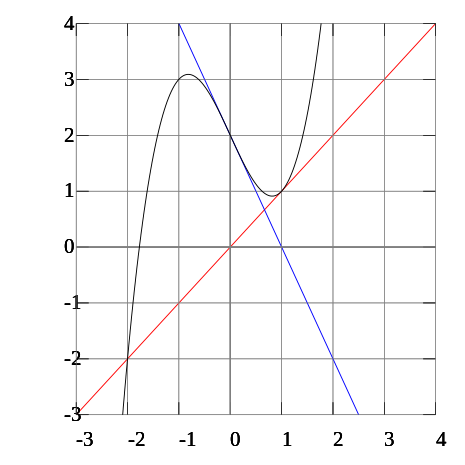
\includegraphics[width=0.7\linewidth]{assets/newton_method_tangent_line}
		\caption{The tangent lines of $x^3  + 2x + 2$ at 0 and 1 intersect the x-axis at $(1, 0)$ and $(0, 2)$ respectively and the solution is a point close to -2. In this case, Newton's method never converges.}
		\text{source: \url{https://en.wikipedia.org/wiki/Newton's_method}}
		\label{fig:newtonmethodtangentline}
	\end{minipage}
\end{figure}

In addition, this method faces challenges in terms of computational intensity and memory usage, leading to its limited popularity because it has to compute the inverse of Hessian matrix H (\ref*{hessian}) of the objective function at each step \cite{optimization}. 

To address these issues, various alternative second-order derivatives methods have been proposed over the years such as \textit{Quasi-Newton method and Stochastic Newton method}. These methods leverage additional Hessian information to enhance the training trajectory across the local curvature of the error surface, facilitating finer hyperparameter tuning and enabling adaptive step size adjustments at different learning stages \cite{newton}.

The \textbf{Quasi-Newton} method's idea is to employ a positive definite matrix \(B\) to approximate the inverse of the Hessian matrix \(H\), simplifying the computational complexity. Moreover, the second-order gradient is not applied in the Quasi-Newton, that's the reason why this method's sometimes better than the Newton method.

The iterative update rule for the Quasi-Newton method is expressed as (in 1-dimensional space, use \(x\)):
\begin{equation}
	x_{t+1} = x_t - \alpha_t B_t^{-1} \nabla f(x_t), \qquad (t>0)
\end{equation}
where:
\begin{align*}
	& f && : \text{the objective function}, \\
	& x_t && : \text{the current estimate of the optimal solution at iteration } t, \\
	& \nabla f(x_t) && : \text{the gradient vector of the objective function at } x_t, \\
	& B_t && : \text{an approximation of the Hessian matrix at iteration } t, \\
	& \alpha_t && : \text{the step size determined through a line search or another optimization strategy}.
\end{align*}

Similarly in multi-dimensional space:
\begin{equation}
	\theta_{t+1} = \theta_t - \alpha_t B_t^{-1} \nabla f(\theta_t)
\end{equation}

The update of \(B_t\) is a crucial aspect of the Quasi-Newton method. Among estimation algorithms, the most well-known formula for updating \(B_t\) is the Broyden-Fletcher-Goldfarb-Shanno (BFGS) update \cite{newton}:
\begin{equation}
	B_{t+1} = B_t + \frac{y_t y_t^T}{y_t^T s_t} - \frac{B_t s_t s_t^T B_t^T}{s_t^T B_t s_t}
\end{equation}

where:
\begin{align*}
	& y_t && = \nabla f(\theta_{t+1}) - \nabla f(\theta_t) \quad \text{(difference in gradients)}, \\
	& s_t && = \theta_{t+1} - \theta_t \quad \text{(difference in parameter vectors)}.
\end{align*}

Therefore, the updated $H_{t+1}$ is:
\begin{equation}
	H_{t+1} = \left(I - \dfrac{s_ty_t^T}{s_t^Ty_t}\right) H_t\left(I - \dfrac{y_ts_t^T}{s_t^Ty_t}\right) + \dfrac{y_ts_t^T}{s_t^Tu_t}
\end{equation}

The BFGS update ensures that \(B_{t+1}\) remains symmetric and positive definite, preserving the positive definiteness of the Hessian approximation. The Quasi-Newton method is known for its effectiveness in solving non-linear optimization problems \cite{optimization}, especially when reducing the computation complexity of $O(N^2)$ \cite{newton}.

Like in the first-order optimization methods, when handling with large-scale data, we should use stochastic approximation algorithms with each step of update based on a relatively small training subset. The \textbf{Stochastic Quasi-Newton} (SQN) method is an optimization algorithm that combines elements of stochastic gradient descent with the quasi-Newton method to solve that mentioned problem.

Online BFGS (oBFGS) is a work in stochastic adaptations of the BFGS method (an variant of BFGS) \cite{oBFGS} \cite{SQNM}. In Online-BFGS, the algorithm updates the inverse Hessian approximation using a sequence of stochastic updates (stochastic gradients instead of full gradients), where each update is based on a single data point or a mini-batch \cite{SQNM}.

The specific update rule for the Hessian approximation in Online-BFGS:
\begin{equation}
	H_{k+1} = (I - \rho_k s_k y_k^T) H_k (I - \rho_k y_k s_k^T) + \rho_k s_k s_k^T
\end{equation}
, where $s_k$ is the vector of parameter updates, $y_k$ is the vector of corresponding gradient updates, and $\rho_k$ is a scalar that normalizes the update.

Denote \(\theta_t\) as the parameter vector at iteration \(t\), \(H_t\) as the inverse Hessian approximation at iteration \(t\), \(g_t\) as the stochastic gradient at iteration \(t\) and \(s_t\) as the parameter update computed using the quasi-Newton method, the algorithm \ref{algo:SQNAlgorithm} represents the Stochastic Quasi-Newton method.


\begin{algorithm}
	\caption{Stochastic Quasi-Newton Method \cite{SQNAlgo}}
	\label{algo:SQNAlgorithm}
	\KwData{Training data, learning rate, maximum iterations, convergence criteria}
	\KwResult{Optimal parameters $\theta$}
	
	\SetAlgoNlRelativeSize{0}
	\SetAlgoNlRelativeSize{-1}
	
	Initialize parameters: $\theta_0$\;
	Initialize inverse Hessian approximation: $H_0$\;
	
	\For{$t=1$ \KwTo \text{max\_iterations}}{
		Randomly sample mini-batch: $D_t$\;
		Compute stochastic gradient: $g_t = \nabla J(\theta_t, D_t)$\;
		Compute parameter update: $s_t = -H_t \cdot g_t$\;
		
		Update inverse Hessian approximation using BFGS formula:\\
		$H_{t+1} = (I - \rho_t s_t g_t^T) H_t (I - \rho_t g_t s_t^T) + \rho_t s_t s_t^T$\;
		
		Update parameters: $\theta_{t+1} = \theta_t + s_t$\;
		
		\If{convergence\_criteria($\theta_t, \theta_{t+1}$)}{
			\textbf{break}\;
		}
	}
	
	\Return{$\theta$}
\end{algorithm}

\subsection{Derivative-free optimization}
Certainly, optimization tasks may be challenging to tackle through gradient-based methods, either because the derivative of the objective function is non-existent or difficult to compute. In such cases, derivative-free optimization becomes a relevant approach \cite{optimization}. There are two mainly types of ideas for this optimization method. One is to employ heuristic algorithms that select strategies based on their historical success rather than systematically deriving solutions. One is to fit an appropriate function according to the samples of the objective function, called coordinate descent method $-$ a typical derivative-free algorithm for multi-variable functions \cite{optimization}. 

The primary different between coordinate descent and gradient descent algorithm is about how they determine the update direction \cite{optimization}. In gradient descent, each update direction is guided by the gradient of the current position, potentially not aligning with any coordinate axis. On the other hand, coordinate descent maintains a fixed optimization direction throughout, bypassing the need to compute the gradient of the objective function. It simplifies calculations by updating along a single axis in each iteration. While coordinate descent is efficient for certain problems, it may struggle with indivisible functions, necessitating the use of an appropriate coordinate system to enhance convergence. For instance, the adaptive coordinate descent method employs principal component analysis to establish a new coordinate system with minimal correlation. However, the coordinate descent method still faces challenges such as that on a serial machine, attempting to optimize problems with more than a few tens of variables is typically impractical, and derivative-free optimization may face limitations, especially when minimizing non-convex functions \cite{derivative-free}.

Before moving on to the other section, Table \ref{Tab:evaluation} summarizes all the key information about the aforementioned optimization methods. The table compares and evaluates the methods based on criteria such as convergence speed, handling of curvature, computational efficiency, applicability to large datasets, global optimization, and the complexity of implementation.

\begin{table}[h]
	\centering
	\caption{Comparation and Evaluation of Optimization Methods}
	\begin{tabular}{|>{\raggedright}p{2.5cm} |>{\raggedright}p{3.5cm} |>{\raggedright}p{3.5cm} |>{\raggedright\arraybackslash}p{3.5cm}|}
		\hline
		Criteria & First-Order Methods & Second-Order Methods & Derivative-Free Methods \\
		\hline
		Convergence Speed & Fast for large datasets & Faster convergence, but computationally expensive & Slower compared to gradient-based methods \\
		\hline
		Handling Curvature & Limited information, may struggle with curvature & Better handling due to curvature information & No explicit handling of curvature, relies on function evaluations \\
		\hline
		Computational Efficiency & Efficient for large datasets & Computationally expensive & Varied, depends on problem characteristics \\
		\hline
		Applicability to Large Datasets & Suitable for large-scale problems & Not suitable for large datasets & Varied, may depend on implementation \\
		\hline
		Global Optimization & May converge to local optima & Can handle global optimization with care & Robust to global optimization, suitable for black-box problems \\
		\hline
		Complexity of Implementation & Relatively simple implementation & More complex due to Hessian calculations & Implementation complexity depends on algorithm \\
		\hline
	\end{tabular}
	\label{Tab:evaluation}
\end{table}

\section{Continual learning and Test production in building a ML solution}
\subsection{Continual learning}
Traditional machine learning models are often designed with the assumption that the underlying data distribution remains static. However, in real-world scenarios, the nature of data is dynamic, and new information continuously emerges. This creates a significant challenge: How can machine learning models adapt to new data and tasks over time without forgetting the knowledge acquired from previous experiences?

Continual Learning, also referred to as lifelong learning or incremental learning, addresses the aforementioned challenge by providing a framework for machine learning models to learn and adapt continuously over time without needing a strict distribution \cite{contlearning}. The goal is to construct intelligent systems that evolve with the ever-changing nature of the data they encounter, making them well-suited for applications in dynamic environments and scenarios where ongoing learning is a necessity.

One significant challenge in Continual Learnning is \textbf{catastrophic forgetting} or catastrophic interference \cite{contlearning}. It arises when adjusting to a new distribution typically leads to a substantial decrease in the capacity to retain information from the previous distributions \cite{catastrophic}. This phenomenon poses a challenge in machine learning and neural networks, as the system may struggle to maintain knowledge acquired from earlier tasks when exposed to new information or distributions.

Continual Learning has diverse applications across various domains, where the ability to adapt and accumulate knowledge over time is crucial, shown in the figure \ref{fig:CLapps}.

\begin{figure}[!htb]
	\begin{minipage}[t]{0.48\textwidth}
		\centering
		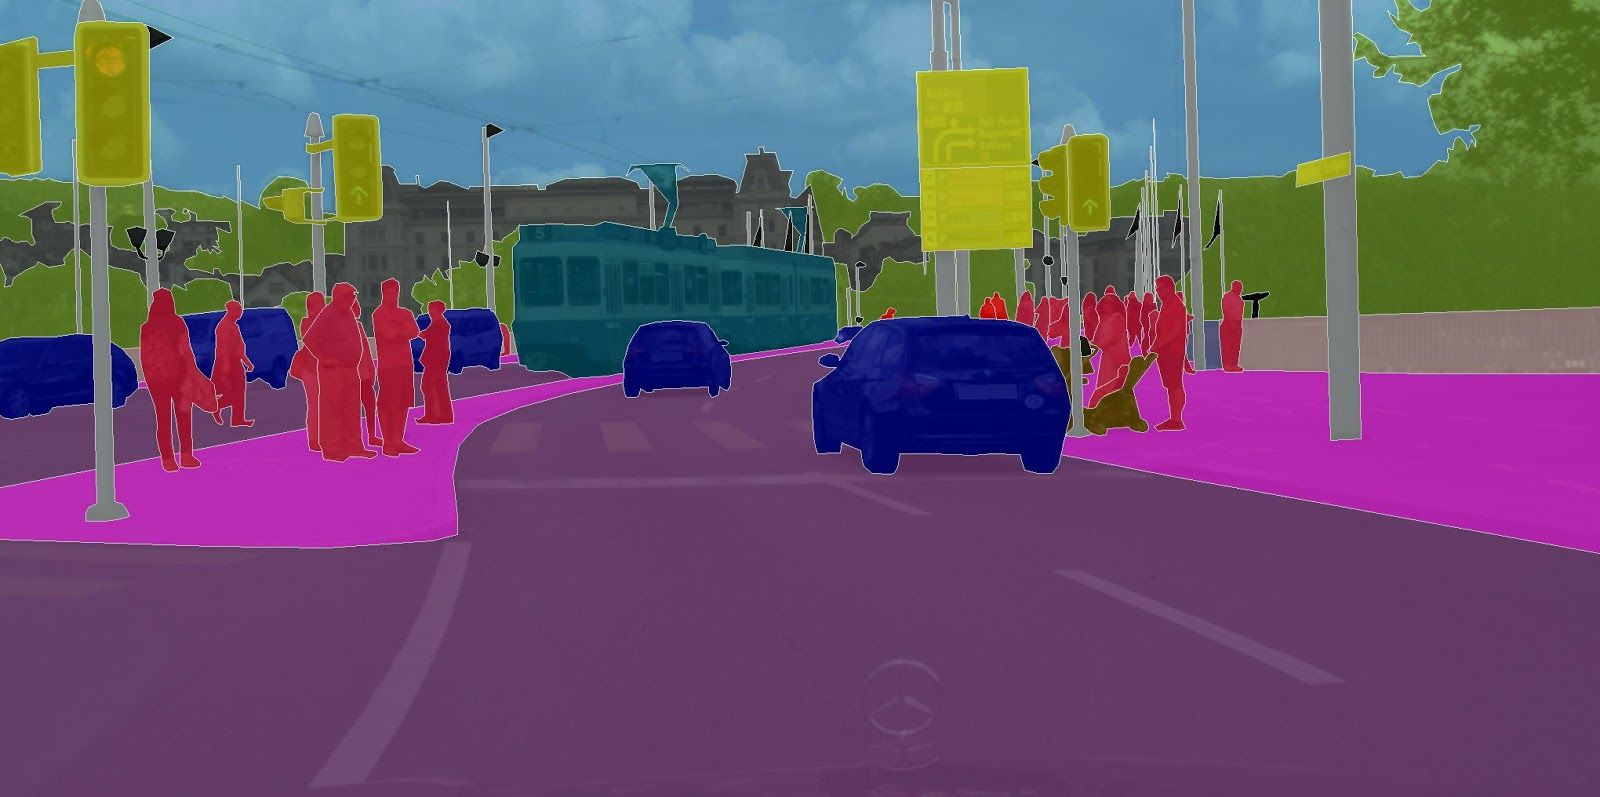
\includegraphics[width=1\linewidth]{assets/semantic_segmentation}
		\label{fig:semanticsegmentation}
	\end{minipage}	
	\begin{minipage}[t]{0.48\textwidth}
		\centering
		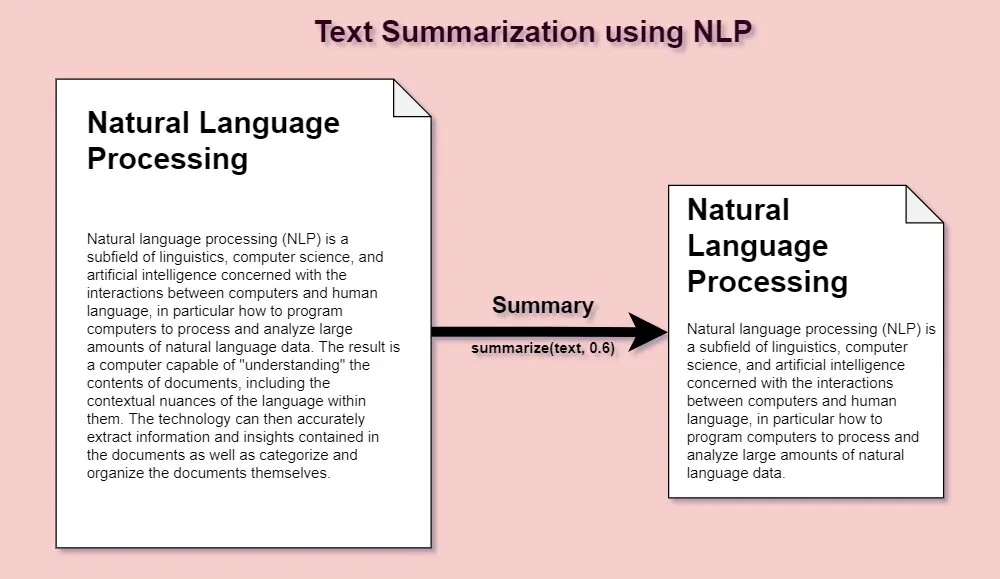
\includegraphics[width=1\linewidth]{assets/text_sum}
		\label{fig:textsum}
	\end{minipage}\hfill
	
	\caption{Some applications of Continual Learning: Semantic Segmentation (left) and Text Summarization (right)}
	\label{fig:CLapps}
\end{figure}

\subsection*{Continual Learning methods}
Continual learning methods encompass a diverse set of strategies aimed at addressing the challenges posed by learning from sequential, non-i.i.d. data streams, shown in the figure \ref{fig:methods}.

\begin{figure}[!htb]
	\centering
	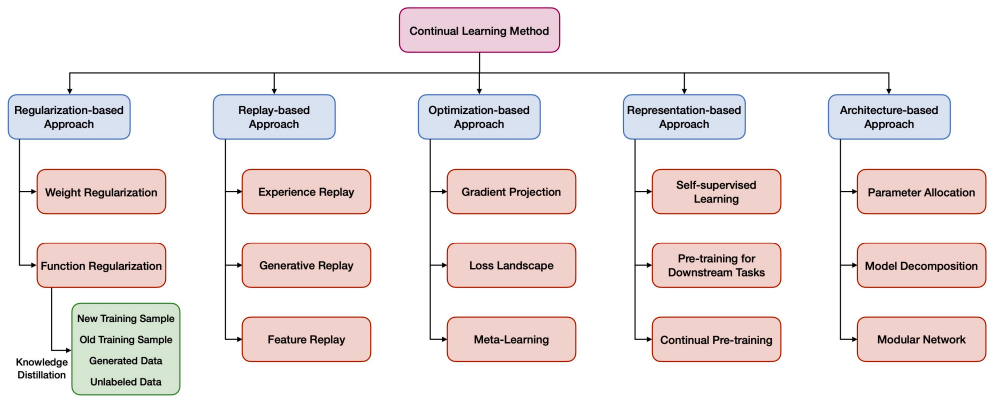
\includegraphics[width=0.8\linewidth]{assets/methods}
	\caption{A state-of-the-art and elaborated taxonomy of representative continual learning methods. We have summarized 5 main categories (blue	blocks), each of which is further divided into several sub-directions (red blocks). \cite{contlearning}}
	\label{fig:methods}
\end{figure}
 

Here's a summary of five prominent continual learning approaches:

\begin{enumerate}
	\item \textbf{Regularization-Based Approach:}
	\begin{itemize}
		\item \textit{Objective:} Mitigate catastrophic forgetting by incorporating regularization terms in the loss function.
		\item \textit{Mechanism:} Penalize significant changes in model parameters to encourage knowledge retention from previous tasks.
		\item \textit{Strengths:} Effective in preventing interference between tasks and stabilizing model updates.
		\item \textit{Considerations:} Careful tuning of regularization hyperparameters is required.
	\end{itemize}
	
	\item \textbf{Replay-Based Approach:}
	\begin{itemize}
		\item \textit{Objective:} Alleviate catastrophic forgetting by storing and replaying samples from past tasks during training.
		\item \textit{Mechanism:} Augment current task data with samples from a memory buffer containing historical data.
		\item \textit{Strengths:} Robust in preserving knowledge from earlier tasks, particularly when combined with other approaches.
		\item \textit{Considerations:} Memory management challenges, scalability concerns, and potential bias in replayed samples.
	\end{itemize}
	
	\item \textbf{Optimization-Based Approach:}
	\begin{itemize}
		\item \textit{Objective:} Optimize the learning process to adapt to new tasks while maintaining proficiency on previous tasks.
		\item \textit{Mechanism:} Dynamically adjust learning rates, task-specific updates, or optimization algorithms during training.
		\item \textit{Strengths:} Adaptable to changing task distributions and varying degrees of task difficulty.
		\item \textit{Considerations:} Complexity in designing adaptive optimization strategies and potential trade-offs between plasticity and stability.
	\end{itemize}
	
	\item \textbf{Representation-Based Approach:}
	\begin{itemize}
		\item \textit{Objective:} Learn task-agnostic and task-specific representations that facilitate continual learning.
		\item \textit{Mechanism:} Train models to extract features that are both generalizable across tasks and specific to individual tasks.
		\item \textit{Strengths:} Enhances model adaptability and transferability of learned representations.
		\item \textit{Considerations:} Balancing the extraction of generic and task-specific features.
	\end{itemize}
	
	\item \textbf{Architecture-Based Approach:}
	\begin{itemize}
		\item \textit{Objective:} Adapt the model's architecture dynamically to accommodate new tasks.
		\item \textit{Mechanism:} Adjust the model's structure (add/remove layers, modules) based on evolving task requirements.
		\item \textit{Strengths:} Enables flexibility in handling diverse tasks and evolving data distributions.
		\item \textit{Considerations:} Increased model complexity and potential challenges in determining optimal architectural changes.
	\end{itemize}
\end{enumerate}


\subsection*{Learning process Formulation} The objective is to minimize the cumulative loss over all encountered tasks while incorporating a regularization term to prevent catastrophic forgetting. And in continual learning, the training samples of each task can arrive incrementally in batches (i.e., $\{D_{t,b}\}_{b \in B_t}^{t \in T}$) or simultaneously (i.e., $\{D_t\}_{t \in T}$) \cite{contlearning}, where:
\begin{align*}
	&D_{t,b} \quad &&\text{: the set of training samples for task $t$ in batch $b$,} \\
	&B_t \quad &&\text{: the set of batches for task $t$,} \\
	&T \quad &&\text{: the set of tasks.}
\end{align*}

By setting $T$ as the tasks $T$, the objective function for task $t$ can be defined as follows:
\begin{equation}
	L_t(\theta) = - \sum_{i=1}^{N_t} y_{i,t} \log(f(x_{i,t};\theta))
\end{equation}
, where:
\begin{align*}
	&L_t(\theta) &:& \text{The objective function for task } t. \\
	&\theta      &:& \text{The parameters of the model, which are adjusted during the learning process.} \\
	&N_t         &:& \text{The number of samples in task } t. \\
	&x_{i,t}     &:& \text{The input for the } i\text{-th sample in task } t. \\
	&y_{i,t}     &:& \text{The corresponding ground truth for the } i\text{-th sample in task } t. \\
	&f(x_{i,t};\theta) &:& \text{The model's prediction for the } i\text{-th sample in task } t.
\end{align*}

The learning algorithm adjusts the model parameters $\theta$ to minimize this task-specific loss, effectively improving the model's ability to perform well on the given task. In Continual Learning, the challenge is not only to minimize the loss for the current task but also to retain knowledge from previous tasks, which is often addressed through additional regularization terms in the overall learning objective.


The regularization term for task \(t\) is a regularization mechanism incorporated into the learning objective to address the challenge of catastrophic forgetting \cite{cont-regular}. It is represented as:
\begin{equation}
	R_t(\theta) = \sum_{i=1}^{t-1} \Omega(\theta, \theta_i)
\end{equation}
, where:
\begin{itemize}
	\item $R_t(\theta)$: The Knowledge Retention Term for task $t$. This term penalizes changes in the model's parameters ($\theta$) concerning the parameters at the initialization of the learning process ($\theta_i$) for tasks $i < t$.
	
	\item $\Omega(\theta, \theta_i)$: A measure of the change in parameters from the initial state $\theta_i$ to the current state $\theta$. The choice of the measure depends on the specific regularization strategy used, and it is designed to capture the extent of modification in the model parameters.
\end{itemize}

In conclusion, the combined objective for continual learning is:
\begin{equation}
	\min_{\theta} \sum_{t \in T} \left( L_t(\theta) + \lambda R_t(\theta) \right)
\end{equation}

\subsection*{Evaluation metrics}

After training a continual learning model, evaluation is an integral part of the model development life cycle. It provides insights into the model's strengths and weaknesses, informs decision-making, and guides further development and refinement efforts. Here is some metrics to assess a classification model particularly.

\begin{enumerate}
	\item \textbf{Overall Performance:}
	Assess the model's performance across all tasks using metrics such as average accuracy (AA), average incremental accuracy (AIA). Consider $a_{k,j} \in [0, 1]$, which represents the classification accuracy assessed on the test set of the $j$-th task after incrementally learning the $k$-th task ($j \leq k$). The calculation of $a_{k,j}$ involves the classes in either $Y_j$ or $\bigcup_{i=1}^{k} Y_i$, depending on whether multi-head evaluation (e.g., TIL) or single-head evaluation (e.g., CIL) [64] is employed \cite{contlearning}. The metrics at the $k$-th task are then defined as:
	\begin{equation}
		AA_k = \frac{1}{k} \sum_{j=1}^{k} a_{k,j},
	\end{equation}
	\begin{equation}
		AIA_k = \frac{1}{k} \sum_{i=1}^{k} AA_i.
	\end{equation}	
	

	\item \textbf{Memory Stability:}
	Evaluate the stability of the model's memory retention over time. This metric measures the degree to which the model preserves knowledge from earlier tasks without interference or forgetting when learning new tasks. The forgetting of a task is calculated by the difference	between its maximum performance obtained in the past and its current performance \cite{contlearning}
	\begin{equation}
		f_{j,k} = \max_{i \in \{1, \ldots, k-1\}} (a_{i,j} - a_{k,j}), \quad \forall j < k
	\end{equation}
	Therefore, the \textit{forgetting measure} (FM) at the $k-th$ task is the average forgetting of all old tasks:
	\begin{equation}
		FM_k = \frac{1}{k-1} \sum_{j=1}^{k-1} f_{j,k}.
	\end{equation}
	
	\item \textbf{Learning Plasticity:}
	Quantify the model's ability to adapt and learn efficiently when faced with new tasks. Learning plasticity reflects how well the model can rapidly adjust to new information without negatively impacting its performance on previously learned tasks, called \textit{intransience measure} (IM) \cite{contlearning}. It follows:
	\begin{equation}
		IM_k = a^*_k - a_{k,k},
	\end{equation}
	, where $a^*_k$ is the classification accuracy of a randomly initialized reference model jointly trained with all the data $\bigcup_{k} \bigcup_{j=1}^{k} D_j$ for the $k$-th task.
	
\end{enumerate}

In conclusion, continual learning is a dynamic approach to machine learning, allowing models to adapt to new tasks while retaining knowledge from past experiences. Its advantages include incremental learning and resource efficiency. However, challenges such as catastrophic forgetting pose significant obstacles. Achieving the right balance between adaptability and knowledge retention remains a key research focus.


\subsection{Test production}

Testing is a critical phase in the development of a machine learning solution, ensuring that the model performs effectively and reliably in real-world scenarios. The test production phase encompasses a series of assessments and evaluations to validate the model's performance, robustness, and its ability to meet the specified objectives. This phase is pivotal in identifying and rectifying any issues before deploying the machine learning solution into a production environment.

\begin{figure}[!htb]
	\centering
	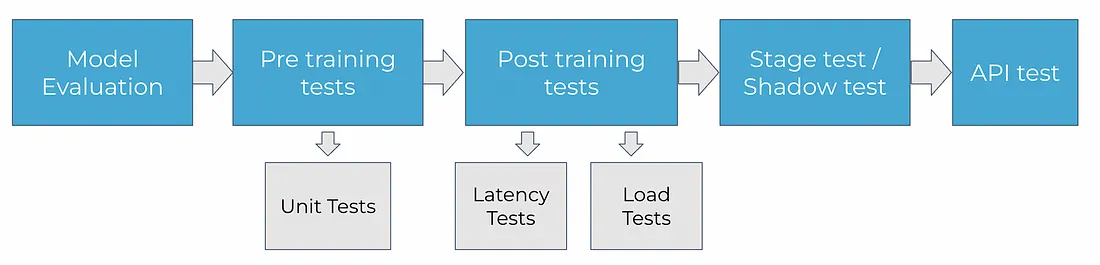
\includegraphics[width=0.65\linewidth]{assets/test-flow}
	\caption{Machine Learning testing flow \cite{test}}
	\label{fig:test-flow}
\end{figure}

The figure \ref{fig:test-flow} above shows a flow of testing in machine learning production. We are going through each step. 

\begin{enumerate}
	\item \textbf{Model evaluation}: In the initial stage of model testing, referred to as model evaluation (stage 0), the focus is on assessing the functionality of the model. Evaluation metrics vary based on the type of model and the nature of the dataset. For classification tasks with imbalanced datasets, F1 scores and AUC scores are considered effective indicators of model quality. In regression tasks dealing with outlier-heavy data, Mean Absolute Error (MAE) proves to be a more suitable metric.
	
	For certain models, particularly ensemble-decision tree-based supervised models like XGBoost and Random Forest (RF), interpretability can be challenging due to their black-box nature. To address this, SHAP (SHapley Additive exPlanations) can be employed to gain insights into the logic behind predictions at an overall level. Additionally, for specific case inspections, LIME (Local Interpretable Model-agnostic Explanations) can be utilized, offering a more granular understanding of individual predictions within these complex models. These interpretability tools enhance the transparency and comprehensibility of model outputs, especially in scenarios where interpretability is crucial.
	
	
	\item \textbf{Pre-training test}: is tests we prepare before training model to check if it is meet the model such as the right format of data, enough data, etc. Here's something we can test:
		\begin{itemize}
			\item[-] Feature Engineering: is to that feature engineering processes are implemented correctly and consistently. Testing on feature engineering includes validating the creation of new features, assessing the encoding of categorical variables, verifying the correct application of scaling or normalization. etc.
			
			\item[-] Input data: is to validate the quality and integrity of input data before it enters the modeling pipeline. Testing on input data includes checking for missing values in the input data, ensuring data types are as expected, etc.
			
			\item[-] Model reproducibility: is to ensure that model training and predictions are reproducible, yielding consistent results across different runs. Testing on model reproducibility includes validating that model hyperparameters and configurations remain constant, confirm the same results with identical input data, etc.
		\end{itemize}
		
	\item \textbf{Post training testing} (summary in the figure \ref{fig:post-test}): In batch learning, post-training tests are conducted after the completion of the training phase, whereas in online learning, these tests occur during training. A significant aspect of model evaluation in online learning is the Latency Test, which ensures that predictions are made within a fraction of a second for scalable and traffic-efficient performance. This is particularly important for online machine-learning approaches. One recommended technique involves setting hyperparameters as static values to prevent latency spikes, with optimal values determined through techniques like random-search cv on sampled datasets. Additionally, Load Testing evaluates the model's ability to handle large volumes of test data simultaneously, applicable to both batch and online learning scenarios. Techniques such as using SQLalchemy for parallel database access, monitoring CPU/memory with AWS containers, and employing tools like Locust for automated load testing contribute to comprehensive model assessment.
	\begin{figure}
		\centering
		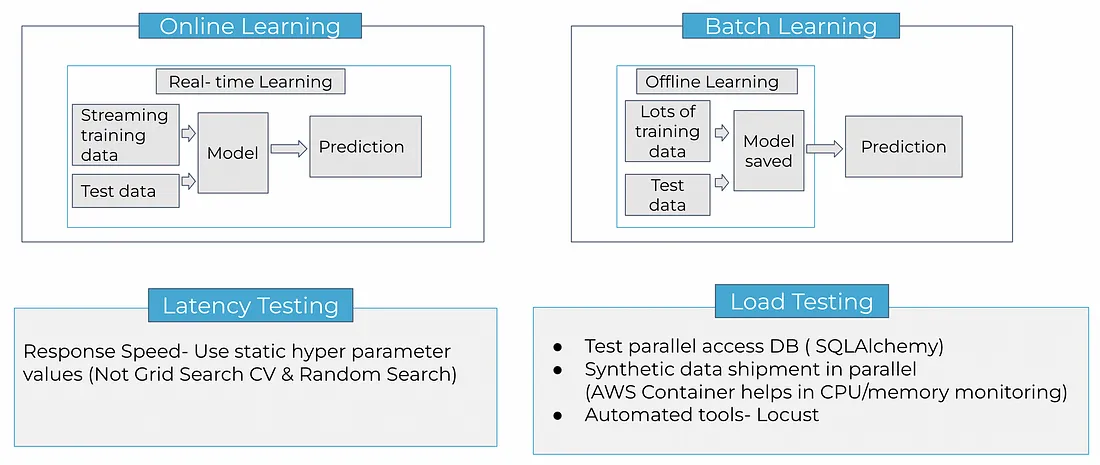
\includegraphics[width=0.8\linewidth]{assets/post-test}
		\caption{Compare online learning and batch learning with respect to the criteria of latency testing and load testing in the post-training test stage. \cite{test}}
		\label{fig:post-test}
	\end{figure}
	
	\item \textbf{A/B testing: Model retraining}: Over time, data features can change, leading to challenges in machine learning (ML) and artificial intelligence (AI) models. \textit{Data drift} occurs when the model trained on older data struggles to perform well with new data, while concept drift arises when the assumptions of a model become invalid in real-world scenarios during deployment. Retraining becomes imperative post-ML deployment to adapt models to evolving conditions. A/B testing, facilitated seamlessly by AWS Sagemaker, serves as a crucial tool in this process. In this testing approach, 80\% of traffic is directed to the current or old ML model, while the remaining 20\% is allocated to the new model (challenger). By comparing their performance based on established baseline metrics, A/B testing helps determine whether the new model should replace the old one, ensuring continuous optimization and effectiveness in real-world applications.
	
	\begin{figure}[!htb]
		\centering
		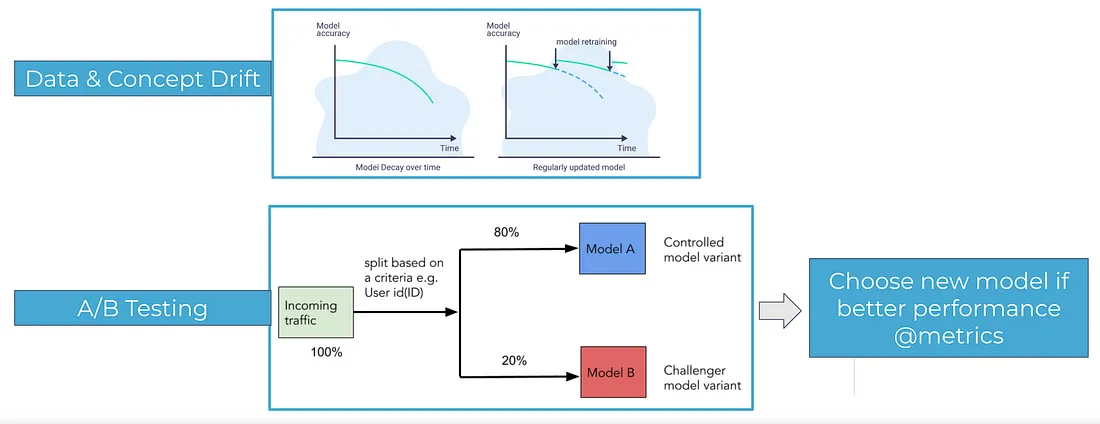
\includegraphics[width=0.8\linewidth]{assets/abtest}
		\caption{A/B Testing steps demonstration}
		\label{fig:abtest}
	\end{figure}
	
	
	\item \textbf{Stage test/Shadow test}: The Stage test is one of the final tests to check whether the model will give the desired output, utilizing diverse test data such as real-world data characteristics. And shadow test is safe way, used when checking on large ML/AI models deployment. The steps in shadow test begins with deploying the new model in parallel with an existing one (if present), then routing each user request to both models for predictions but only serve the output from the existing model to the user, the other will be used for model evaluating.
	
	\item \textbf{API (Application Programming Interface) testing} This is the final stage, mainly focusing on how the actual end-users will experience the responses from the model. The primary goal of this testing phase is to simulate real-world user interactions with the model through its API.
	
\end{enumerate}

\pagebreak


\begin{thebibliography}{9}
	

\bibitem{optimization}
	Shiliang Sun and et al (2019), \emph{A Survey of Optimization Methods from a Machine Learning Perspective}, arXiv.

\bibitem{GD}
	S. Ruder (2016), \emph{An overview of gradient descent optimization algorithms}, arXiv.
		
\bibitem{SGD}
	Christopher M. Bishop (2006), \emph{Pattern Recognition and Machine Learning} (pp. 240-241), Springer Science+Business Media.
	
\bibitem{videocls}
	A. Karpathy and G. Toderici (2014), \emph{Large-scale video classification with convolutional neural networks}, in IEEE Conference on Computer Vision and Pattern Recognition.
	
\bibitem{LSDDeepNet}
	Jeffrey Dean, Greg S. Corrado and et al (2012), \emph{Large Scale Distributed Deep Networks}, in NIPS 2012: Neural Information Processing Systems.
	
\bibitem{newton}
	Hong Hui Tan and King Hann Lim (2019), \emph{Review of second-order optimization techniques in
		artificial neural networks backpropagation}, in IOP Conf. Ser.: Mater. Sci
		
\bibitem{oBFGS}
	N. N. Schraudolph, J. Yu, and S. Gunter, (2007) \emph{A stochastic quasi-Newton method for online convex optimization} (pp. 436–443) in Artificial Intelligence and	Statistics.
		
\bibitem{SQNM}
	Guo, TD., Liu, Y. and Han, CY (2023), \emph{An Overview of Stochastic Quasi-Newton Methods for Large-Scale Machine Learning} in J. Oper. Res. Soc. China.
	
\bibitem{SQNAlgo}
	R. H. Byrd, S.L. Hansen, Jorge Nocedal, and Y. Singer (2015), \emph{A Stochastic Quasi-Newton Method for Large-Scale Optimization}, arXiv.
	
\bibitem{derivative-free}
	A. R. Conn, K. Scheinberg, and L. N. Vicente (2009), \emph{Introduction to Derivative-Free Optimization} (pp. 5-6) in Society for Industrial and Applied Mathematics.
	
\bibitem{contlearning}
	Liyuan Wang, and et al (2015), \emph{A Comprehensive Survey of Continual Learning: Theory, Method and Application}, arXiv.

\bibitem{catastrophic}
	Robert M. French (1999), \emph{Catastrophic Forgetting in Connectionist Networks:Causes, Consequences and Solutions}, Trends in Cognitive Sciences.
	
\bibitem{cont-regular}
	Hongjoon Ahn, Sungmin Cha, Donggyu Lee and Taesup Moon (2019), \emph{Uncertainty-based Continual Learning with Adaptive Regularization}, arXiv.
	
\bibitem{test}
	Shivika K Bisen (May 20, 2023) \emph{Machine Learning Model Testing for Production} in Bright ML, \href{https://medium.com/bright-ml/machine-learning-artificial-intelligence-testing-for-production-c561590ff292}{medium.com/bright-ml/machine-learning-artificial-intelligence-testing-for-production}

\end{thebibliography}

\end{document}